\section{User interface}

\subsection{Structure}

A small overview of the menu Structure.

\subsubsection{Start screen}

When the app is launched, the user will first enter the start screen. It features a menu where the user can choose which functionality to enter: \\
Either to record new data, to view the recorded data in the web application or to enter the settings screen where the sensor device can be scanned for and connected to.

%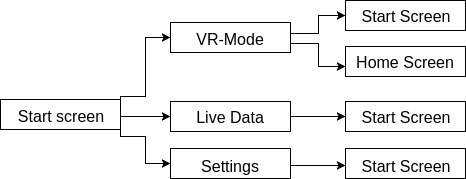
\includegraphics[scale=0.5]{pics/startscreen.jpg}

\subsubsection{VR Mode}

The VR mode normally launches in normal 3D mode from where the user can switch to stereoscopic 3D view.

%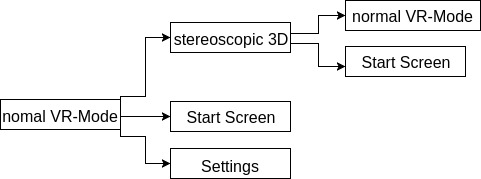
\includegraphics[scale=0.5]{pics/Vr-Mode.jpg}

\subsubsection{Record Data}

Here, new data can be recorded as part of a new set of data or as part of an existing data set.

%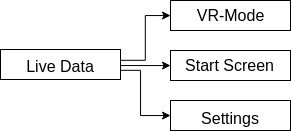
\includegraphics[scale=0.5]{pics/Live_Data.jpg}


\subsubsection{Settings}

Here the user can select which sensor in range he wants to connect to and some basic settings like switching Bluetooth on and off and scan for more devices.

%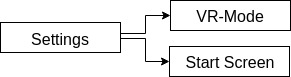
\includegraphics[scale=0.5]{pics/Settings.jpg}

%\subsection{Layout}

%A mockup of the Start up screen. 
%\\
%\\
%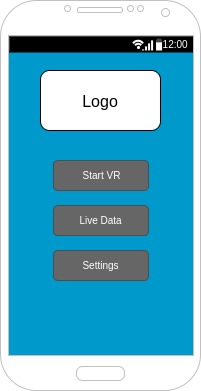
\includegraphics[scale=0.5]{pics/startScreen_mockup.jpg}
%\\

%And a mockup of the stereoscopic Vr-Mode.
%\\
%\\
%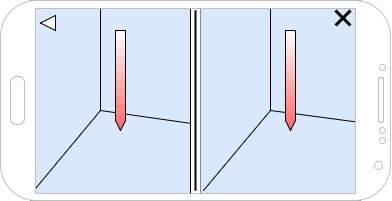
\includegraphics[scale=0.5]{pics/VRView_mockup.jpg}
